\bookchapter{Random Variables and Expected Value}\label{ch:rv}

\section*{Explanation}
Until now events were ``goal'' or ``miss''. For calculations we want \emph{numbers}: how many goals in ten kicks, how much reward, how far away is the ball. A \textbf{random variable} $X$ is a number that depends on the outcome of a random experiment. Its value is not known in advance, but we know how likely each value is.

\subsection*{Probability distribution of a discrete variable}
A random variable that takes only separate values (a count, a die) is \textbf{discrete}. Its \textbf{probability distribution} lists every value $x$ with its probability $P(X=x)$. The probabilities are $\ge0$ and add up to $1$.

\begin{example}
Let $X$ be the number shown by a fair die: $P(X=x)=\frac16$ for $x=1,\dots,6$. Let $Y$ be the reward of a robot in a drill: $0$ points with probability $0.2$, $1$ point with $0.5$, $3$ points with $0.3$.
\begin{center}
\renewcommand{\arraystretch}{1.15}
\begin{tabular}{c|ccc}
$y$ & 0 & 1 & 3\\ \hline
$P(Y=y)$ & 0.2 & 0.5 & 0.3
\end{tabular}
\end{center}
\end{example}

\subsection*{Expected value}
The \textbf{expected value} (mean) $E[X]$ is the average of the values, \emph{weighted} by their probabilities:
\[
E[X]=\sum_x x\cdot P(X=x).
\]
It is the value that you get on average in the long run (law of large numbers, Figure~\ref{fig:pr1_conv}). It does not have to be a value that can really occur.

For the die: $E[X]=\frac16(1+2+3+4+5+6)=3.5$. For the drill reward: $E[Y]=0\cdot0.2+1\cdot0.5+3\cdot0.3=1.4$.

\begin{center}
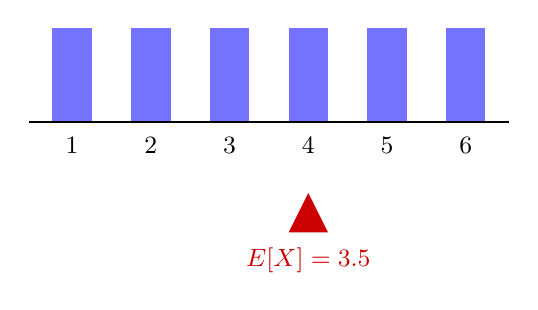
\begin{tikzpicture}
  \foreach \dv in {1,...,6}{
    \fill[blue!55] (\dv,0) rectangle ++(0.5,{1.2});
    \node[font=\small] at (\dv+0.25,-0.3) {\dv};
  }
  \draw[thick] (0.7,0) -- (6.8,0);
  \fill[red!80!black] (4.25,-0.9) -- (4.0,-1.4) -- (4.5,-1.4) -- cycle;
  \node[font=\small,red!80!black] at (4.25,-1.75) {$E[X]=3.5$};
\end{tikzpicture}
\captionof{figure}{The expected value is the balance point of the distribution. All six faces have the same weight, so the balance point of the die lies in the middle at $3.5$.}\label{fig:pr3_balance}
\end{center}

\begin{example}[Which kick is better?]
Kick~A scores with probability $0.3$ and gives $+10$ points for a goal and $-1$ for a miss. Kick~B is safer: it scores with probability $0.9$ but gives only $+5$ for a goal and $-1$ for a miss.
\[
E_A=0.3\cdot10+0.7\cdot(-1)=2.3,\qquad E_B=0.9\cdot5+0.1\cdot(-1)=4.4.
\]
On average kick~B is better, although each single kick~A pays more. Comparing choices by their expected reward is exactly what reinforcement learning does (Chapter~\ref{ch:rl1}).
\end{example}

\subsection*{Variance and standard deviation}
Two robots can have the same mean and still behave very differently: one is always close to the mean, the other is wildly inconsistent. The \textbf{variance} measures the typical squared distance from the mean $\mu=E[X]$:
\[
\mathrm{Var}(X)=E\bigl[(X-\mu)^2\bigr]=\sum_x (x-\mu)^2P(X=x)=E[X^2]-\mu^2.
\]
The \textbf{standard deviation} $\sigma=\sqrt{\mathrm{Var}(X)}$ has the same unit as $X$ and is easier to interpret.

For the drill reward $Y$ with $\mu=1.4$: $\mathrm{Var}(Y)=0.2\cdot1.4^2+0.5\cdot0.4^2+0.3\cdot1.6^2=0.392+0.08+0.768=1.24$ and $\sigma=1.11$. For the die: $\mathrm{Var}(X)=\frac{35}{12}=2.92$, $\sigma=1.71$. (Check with the second formula: $E[X^2]=\frac{91}{6}=15.17$, $15.17-3.5^2=2.92$.)

\subsection*{Calculating with random variables}
For constants $a$ and $b$, and two random variables $X$ and $Y$:
\begin{align*}
E[aX+b]&=a\,E[X]+b, & \mathrm{Var}(aX+b)&=a^2\,\mathrm{Var}(X),\\
E[X+Y]&=E[X]+E[Y], & \mathrm{Var}(X+Y)&=\mathrm{Var}(X)+\mathrm{Var}(Y)\ \ \text{if $X,Y$ independent.}
\end{align*}
Adding a constant shifts the mean but does not change the spread. Multiplying by $a$ multiplies the standard deviation by $|a|$. The variances of independent variables \emph{add}: noise accumulates. If a measurement of a distance has $\sigma=2$\,cm and a second independent one $\sigma=3$\,cm, the sum has the variance $4+9=13$, i.e.\ $\sigma=\sqrt{13}=3.6$\,cm, not $5$\,cm.

\subsection*{Two important distributions}
\textbf{Bernoulli.} One kick that scores with probability $p$. We write $X=1$ for a goal and $X=0$ for a miss. Then $E[X]=p$ and $\mathrm{Var}(X)=p(1-p)$. For $p=0.7$: $\mu=0.7$, $\mathrm{Var}=0.21$, $\sigma=0.46$.

\textbf{Binomial.} The number $K$ of goals in $n$ independent kicks with the same probability $p$ is \emph{binomially distributed}:
\[
P(K=k)=\binom nk\,p^k(1-p)^{n-k},\qquad E[K]=np,\qquad\mathrm{Var}(K)=np(1-p).
\]
The factor $\binom nk$ counts the orders in which the $k$ goals can happen (Chapter~\ref{ch:prob}), the rest is the probability of one such order.

\begin{example}
Ten penalties with $p=0.7$. The probability of exactly $7$ goals is $\binom{10}{7}0.7^7\cdot0.3^3=120\cdot0.0824\cdot0.027=0.267$. The expected number is $np=7$ with $\sigma=\sqrt{10\cdot0.7\cdot0.3}=1.45$. The probability of at least $9$ goals is $P(9)+P(10)=0.121+0.028=0.149$: a perfect shootout is not even a rare event, but it is only one in seven.
\end{example}

\begin{center}
\begin{tikzpicture}
\begin{groupplot}[group style={group size=3 by 1,horizontal sep=0.9cm,y descriptions at=edge left}, grn, width=5.1cm,height=4.4cm, xlabel near ticks, ylabel near ticks, xmin=-0.7,xmax=10.7, ymin=0,ymax=0.31, xtick={0,5,10}, ytick={0,0.1,0.2,0.3}, axis lines=left, xlabel={goals $k$}]
  \nextgroupplot[title={\small $p=0.3$}, ylabel={$P(K=k)$}, ybar, bar width=4pt]
  \addplot[fill=blue!55,draw=blue!60!black] coordinates {(0,0.0282)(1,0.1211)(2,0.2335)(3,0.2668)(4,0.2001)(5,0.1029)(6,0.0368)(7,0.009)(8,0.0014)(9,0.0001)(10,0.0)};
  \nextgroupplot[title={\small $p=0.5$}, ybar, bar width=4pt]
  \addplot[fill=blue!55,draw=blue!60!black] coordinates {(0,0.001)(1,0.0098)(2,0.0439)(3,0.1172)(4,0.2051)(5,0.2461)(6,0.2051)(7,0.1172)(8,0.0439)(9,0.0098)(10,0.001)};
  \nextgroupplot[title={\small $p=0.7$}, ybar, bar width=4pt]
  \addplot[fill=blue!55,draw=blue!60!black] coordinates {(0,0.0)(1,0.0001)(2,0.0014)(3,0.009)(4,0.0368)(5,0.1029)(6,0.2001)(7,0.2668)(8,0.2335)(9,0.1211)(10,0.0282)};
\end{groupplot}
\end{tikzpicture}
\captionof{figure}{Binomial distributions for $n=10$ kicks. The centre of each distribution is at $np$ ($3$, $5$ and $7$). The most spread out case is $p=0.5$.}\label{fig:pr3_binom}
\end{center}

\begin{aibox}
In reinforcement learning the \textbf{return} $G$ of an episode is a random variable (because the world is random), and the robot maximises the \emph{expected} return $E[G]$ (Part~VII). Variance matters too: a policy with the same $E[G]$ but a huge variance (sometimes a great kick, mostly a fall) is risky and hard to learn. Sensor noise, too, is modelled as a random variable with mean $0$.
\end{aibox}

\section*{Practice problems}
\begin{enumerate}[label=\textbf{\thechapter.\arabic*}]
  \item A variable $Y$ has $P(Y=0)=0.2$, $P(Y=1)=0.5$, $P(Y=3)=0.3$. Verify $E[Y]=1.4$, and compute $E[Y^2]$, $\mathrm{Var}(Y)$ and $\sigma$.
  \item A game costs $2$ points per roll of a die. You win $12$ points if the die shows a $6$ and nothing otherwise. Compute the expected \emph{net} gain per roll. Is the game fair?
  \item Kick~A: goal probability $0.3$, $+10$ for goal, $-1$ for a miss. Kick~B: probability $0.9$, $+5$, $-1$. A third kick~C has goal probability $0.6$, $+8$ for a goal and $-2$ for a miss. Which one has the highest expected reward?
  \item $E[X]=4$ and $\mathrm{Var}(X)=3$. Compute $E[2X+1]$, $\mathrm{Var}(2X+1)$ and the standard deviation of $2X+1$.
  \item Two independent distance sensors have standard deviations $0.3$\,m and $0.4$\,m. What is the standard deviation of the \emph{sum} of the two errors?
  \item For a Bernoulli variable with $p=0.7$ compute the mean, the variance and the standard deviation.
  \item $K$ is binomial with $n=5$ and $p=0.7$. Find $P(K=4)$, $P(K\ge4)$ and $E[K]$.
  \item A fair coin is tossed $20$ times. Give the expected number of heads and the standard deviation. What is the probability of exactly $10$ heads? (Use $\binom{20}{10}=184\,756$.)
  \item A sensor fails in each hour independently with probability $0.01$. Find the expected number of failures in $200$ hours, and the probability of no failure at all.
  \item[\textbf{\thechapter.10}$\star$] For the die, show that $E[X^2]-\mu^2=\frac{35}{12}$, where $E[X^2]=\frac16(1+4+9+16+25+36)$.
\end{enumerate}
